\section{\texttt{AdmissionManager}}

Your company has been tasked to develop a system that handles the admission applications that parents send, on behalf of their children, to the high schools of a metropolitan
area. Parents can send admission applications to multiple schools. Before sending an application, they must register their child in the system; the registration includes 
login credentials (username and password), the personal data of the child (first name, last name, birthdate, etc.), the name of at least one parent, contact information 
(which must include an email address and a phone number), the name of the last school they attended, and the list of grades (which includes the obtained score, from 1 to 10, 
for each subject). Each application is assigned an identifier by the system, to allow parents to check its status after sending it (which can be “accepted”, “rejected”, or 
“not evaluated”). Parents can withdraw applications previously sent. They can also ask the system to be notified by email when the outcome of the evaluation of an application
is available. School administrators use the system to check the applications sent to their schools and to approve/reject them. In particular, they can retrieve the list of 
applications sent to their schools that have yet to be evaluated; they can also leave comments on the applications, and they can decide to accept or reject the applications.
Administrators can also set a preference to receive a notification, in the form of an email, when a new application is sent to their school.
\begin{enumerate}
    \item Define the goals for the \texttt{AdmissionManager} system.
    \item Select one of the goals defined in the previous point and define in natural language suitable domain assumptions and requirements to guarantee that the 
        \texttt{AdmissionManager} system fulfills the selected goal.
    \item Draw a UML Use Case Diagram describing the main use cases of the \texttt{AdmissionManager} system.
    \item Pick one of the use cases, and define it. 
\end{enumerate}

\paragraph*{Solution}
\begin{enumerate}
    \item The goals are world phenomena shared between the machine and the real world. They are problem of the real world that the \texttt{AdmissionManager} needs to address. We have 
        four examples, which are: 
        \begin{itemize}
            \item User sends an application.
            \item User withdraws an application.
            \item School administrator evaluates an application.
            \item User is notified about an application evaluation. 
        \end{itemize}
        The problem with those goals is that they are only on world side, so they are not well formulated. The term user is ambiguous, it needs to be specified (parents and school 
        administrator). The formulation can be changed to make them correct: 
        \begin{itemize}
            \item Parents can manage (send and then monitor) applications to schools on behalf of their children.
            \item School administrators can manage (check and approve/reject) applications sent to their schools.
        \end{itemize}
    \item A domain assumption like "as soon as an application arrives to the system, a status needs to be assigned to it" is not correct because the status depend on a method in 
        the program and not on something that is granted by the real world. Examples of correct domain assumption, that are not well formulated are: 
        \begin{itemize}
            \item Parents must be registered into the system to issue an application. 
            \item The system must allow parents to register by providing their email address and personal information.  
        \end{itemize}
        In the end, for the first goal we have the following domain assumptions: 
        \begin{itemize}
            \item \texttt{AdmissionManager} allows system administrators to open application windows for their schools.
            \item \texttt{AdmissionManager} allows parents to register into the system and provide contact information and information about their child. 
            \item \texttt{AdmissionManager} allows parents to log into the system using the credentials input at registration time.
            \item \texttt{AdmissionManager} allows parents to indicate in their profile that they want to be notified when the outcome of an application is available. 
            \item \texttt{AdmissionManager} allows parents to send an application to a school. 
            \item \texttt{AdmissionManager} assigns a unique identifier to each application received. 
            \item \texttt{AdmissionManager} allows parents to see the list of applications sent.
            \item \texttt{AdmissionManager} allows parents to withdraw an application previously sent.
        \end{itemize}
        The assumption is the following: 
        \begin{itemize}
            \item Parents provide correct information (in particular, contact information) when registering.
        \end{itemize}

        And for the second goal we have the following domain assumptions: 
        \begin{itemize}
            \item \texttt{AdmissionManager} allows system administrators to insert new administrators in the system and associate them with the corresponding school.
            \item \texttt{AdmissionManager} allows school administrators to log into the system using the credentials assigned to them by system administrators.
            \item \texttt{AdmissionManager} allows school administrators to indicate in their profile that they want to be notified when new applications for their schools are received.
            \item \texttt{AdmissionManager} allows school administrators to retrieve applications (related to their schools) that have yet to be evaluated.
            \item \texttt{AdmissionManager} allows school administrators to select an application yet to be evaluated and leave a comment in it. 
            \item \texttt{AdmissionManager} allows school administrators to accept/reject an application. 
        \end{itemize}
        The assumption is the following: 
        \begin{itemize}
            \item School administrators periodically evaluate applications and guarantee to explicitly accept/reject all applications arrived within the notification window.
        \end{itemize}
    \item The UML use case diagram is the following: 
        \begin{figure}[H]
            \centering
            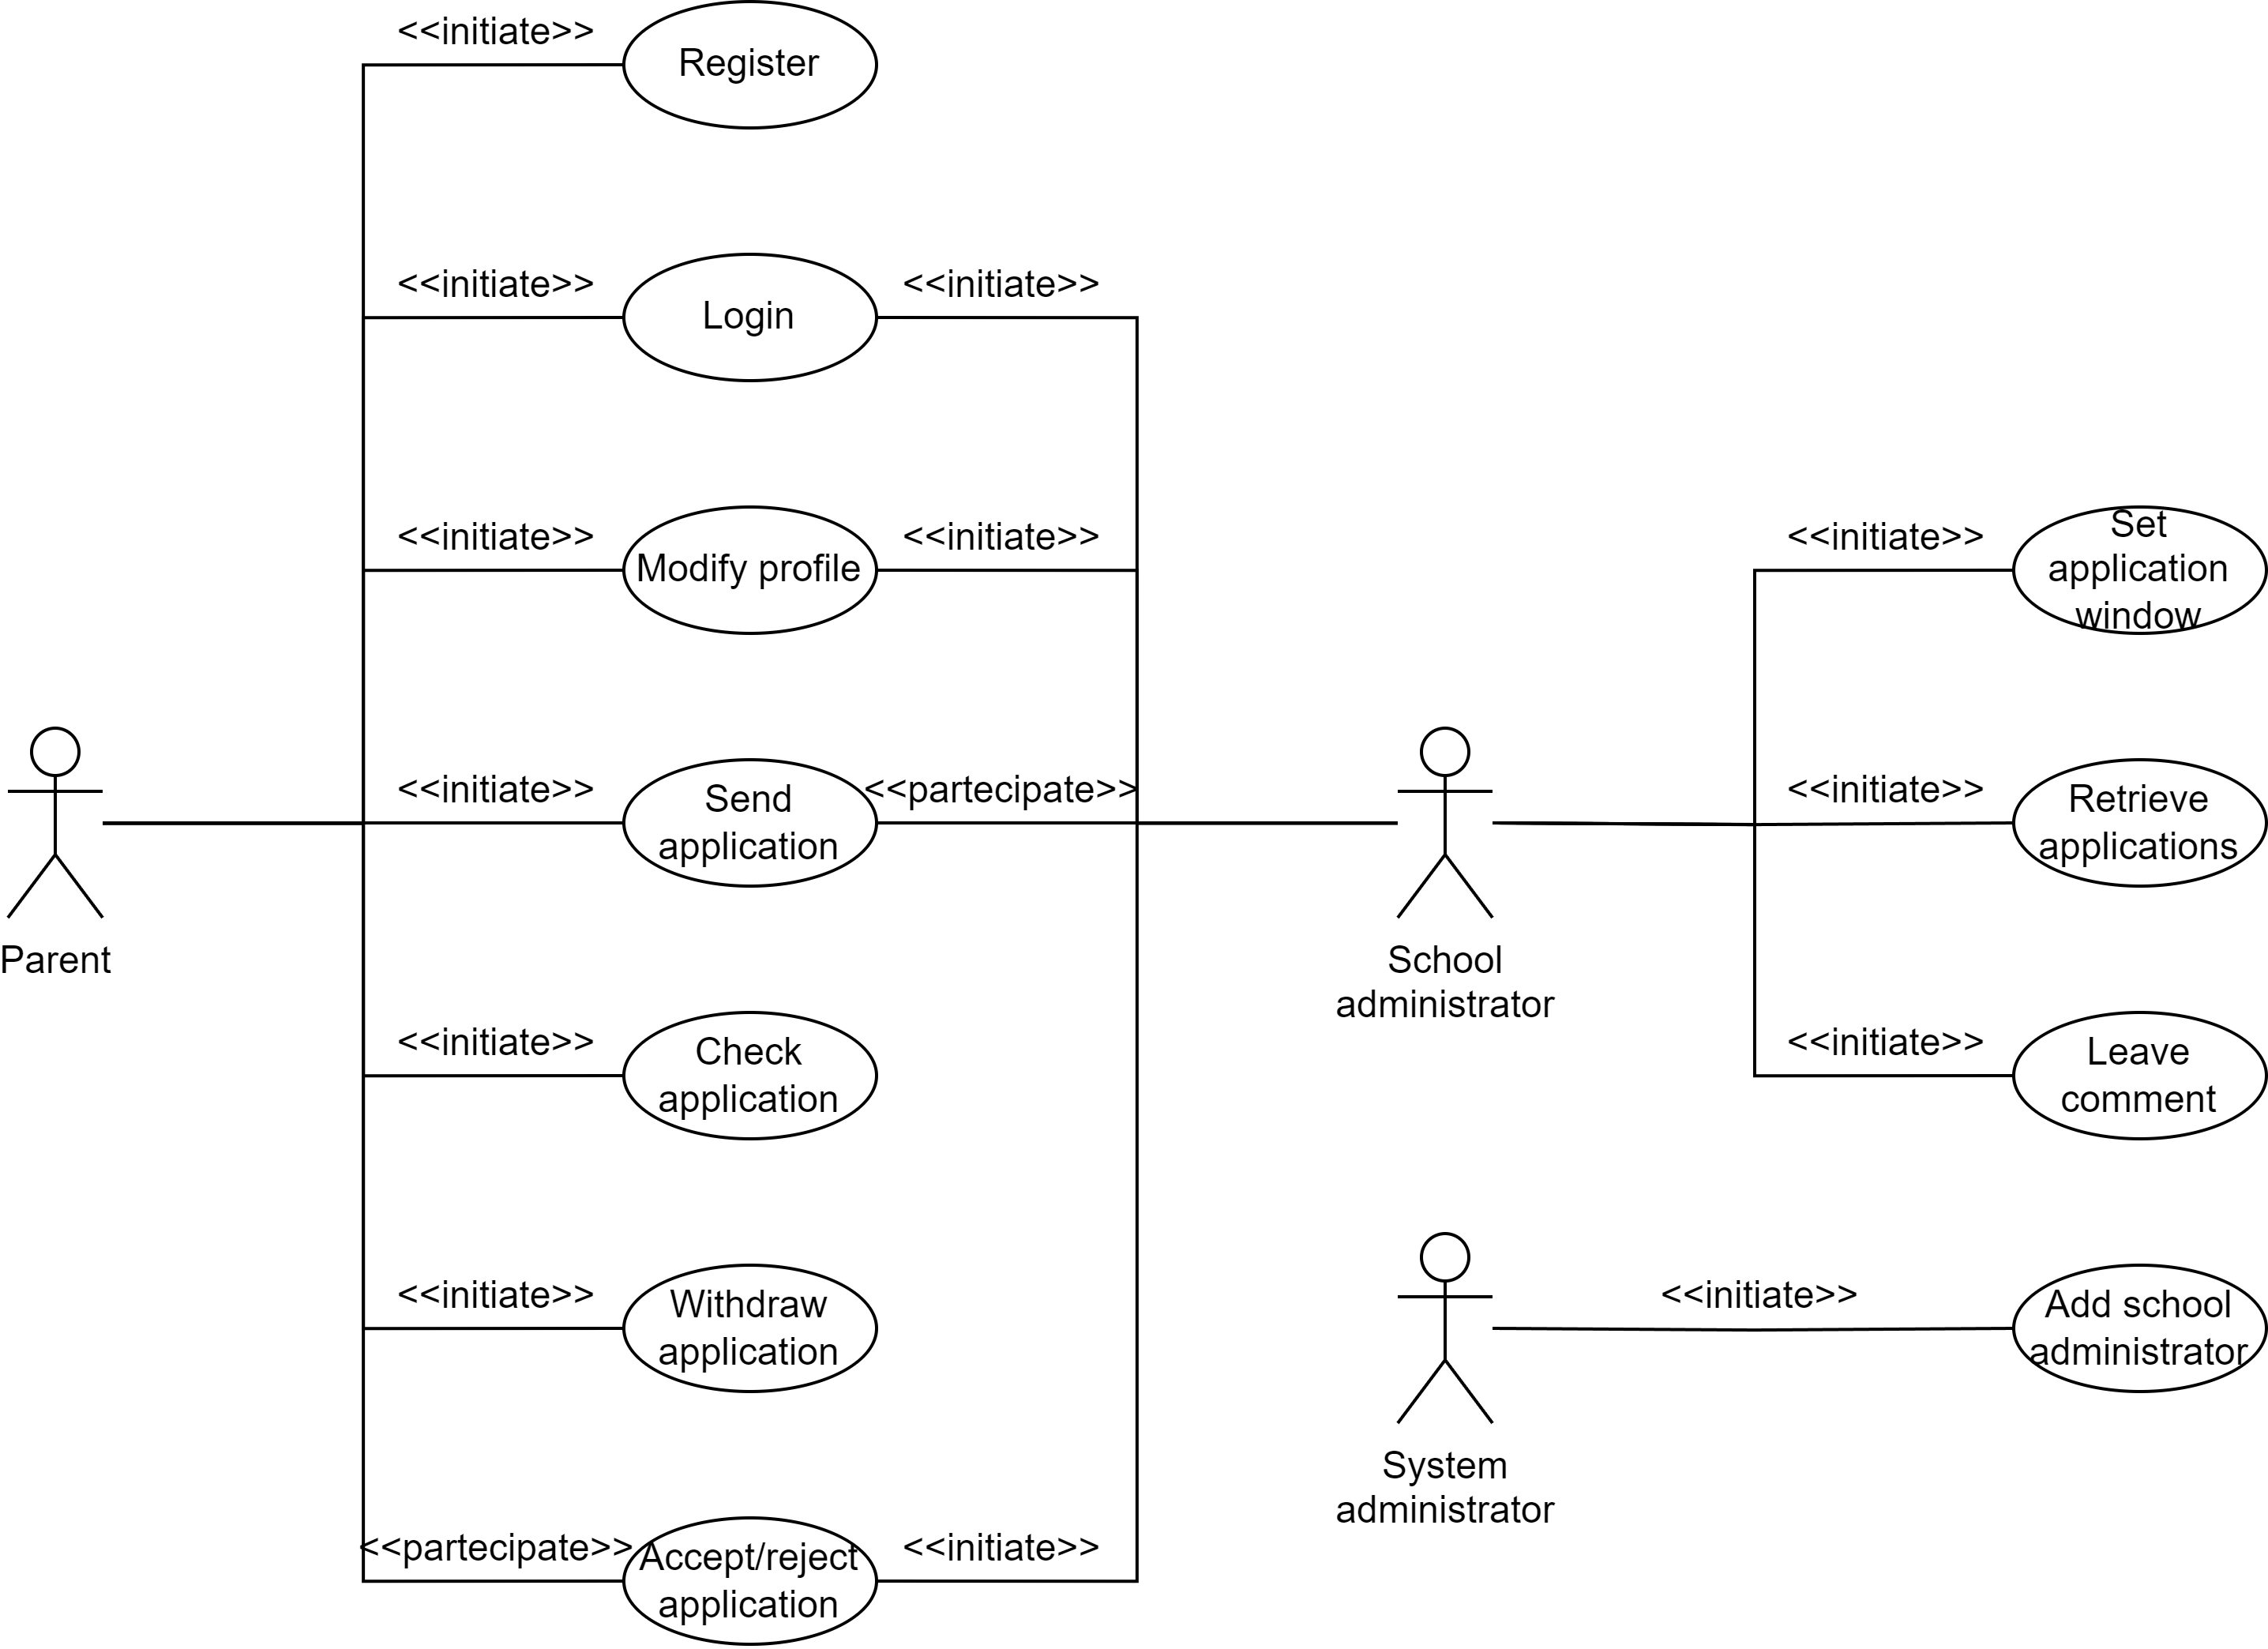
\includegraphics[width=1\linewidth]{images/usecase.png}
        \end{figure}
    \item We select send application case. We have that: 
        \begin{figure}[H]
            \centering
            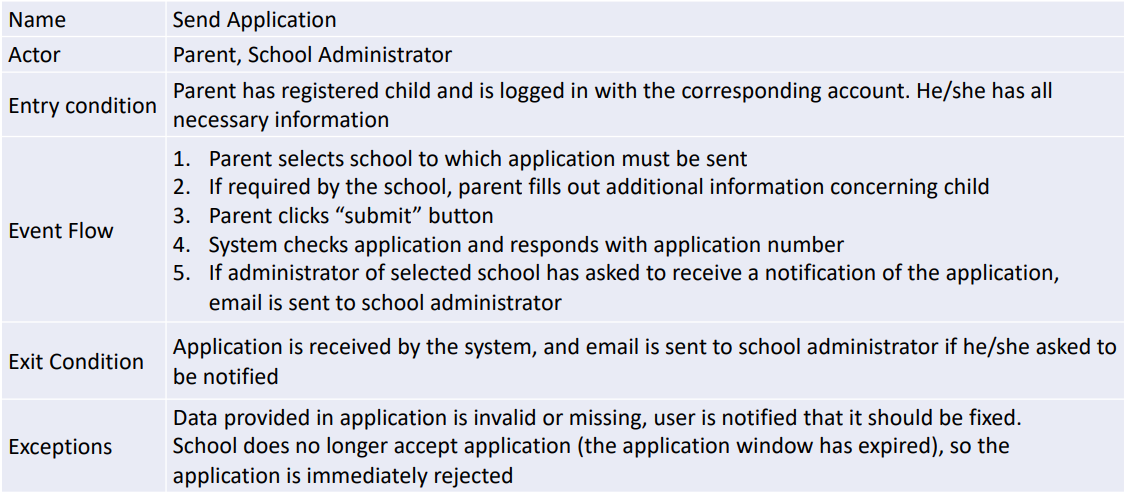
\includegraphics[width=0.9\linewidth]{images/sendapplication.png}
        \end{figure}
\end{enumerate}